\subsection{Diagrammi del package com.sirius.sequenziatore.server}
\begin{figure}[H] \centering 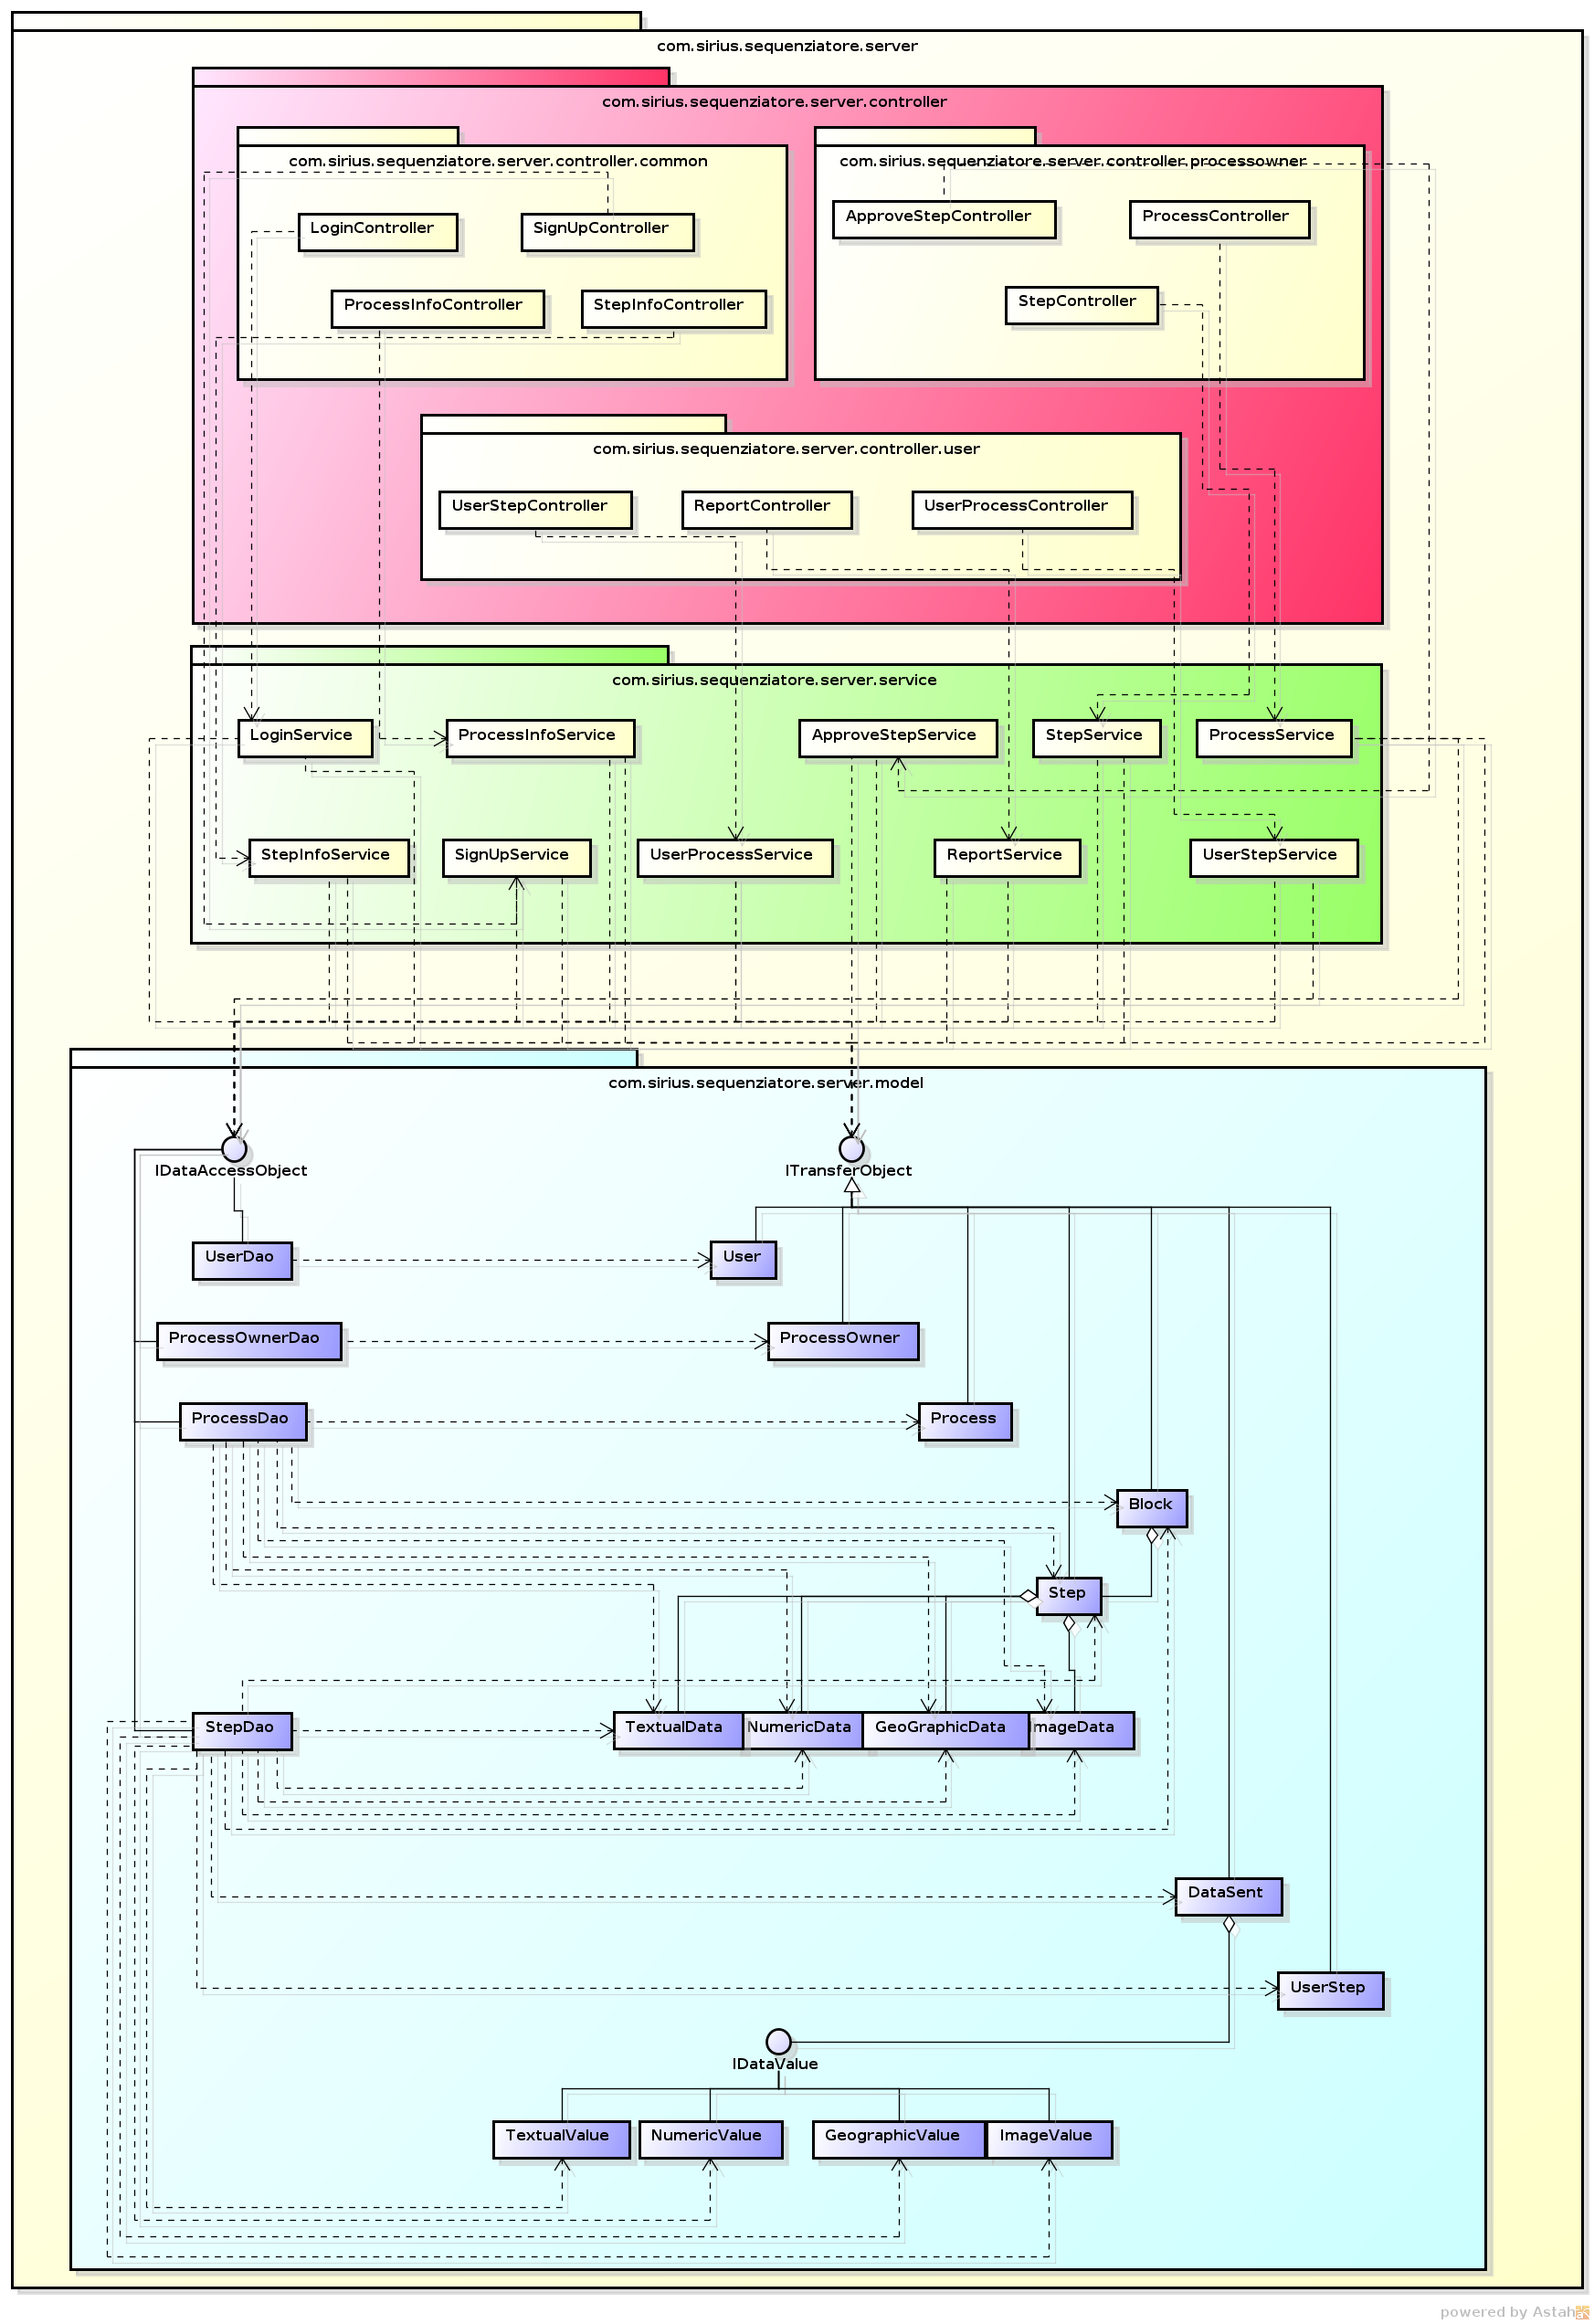
\includegraphics[width=%
\textwidth]
{./pack/server.png} \caption{Diagramma package server}
\end{figure}
Nelle successive sezioni verranno trattati i package del server, come si può notare dal seguente diagramma sono stati rappresentati con tre colori diversi i package controller,service e model in quanto rappresentano i tre tier che compongono il server.
\subsection{Package com.sirius.sequenziatore.server.controller}
\begin{figure}[H] \centering 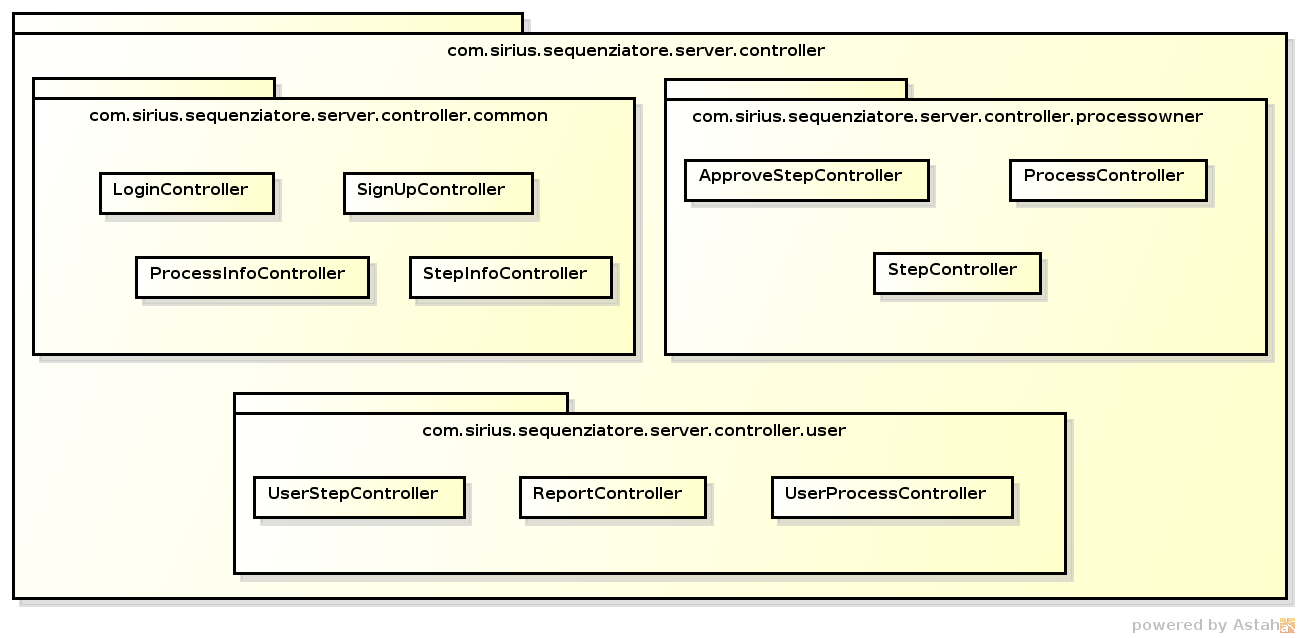
\includegraphics[width=%
\textwidth]
{./pack/servercontroller.png} \caption{Diagramma package controller del server}
\end{figure}
\subsubsection{Package com.sirius.sequenziatore.server.controller.common}
Questo \textit{package} contiene le classi che effettuano operazioni generali oppure comuni tra \textit{Process Owner} e Utenti.
\paragraph{LoginController}
	\begin{itemize}
		\item \textbf{Nome:} \texttt{LoginController};
		\item \textbf{Package:} \texttt{com.sirius.sequenziatore.server.controller.common}
		\item \textbf{Descrizione:} Classe che riceve la richiesta di login di un utilizzatore del sistema, e ritorna l' esito dell' elaborazione del \textit{service} avvisando se l' utente loggato è un \textit{process owner} o un utente normale;
		\item \textbf{Relazione con altre componenti:} la classe invoca i metodi della classe:
		\begin{itemize}
			\item \texttt{com.sirius.sequenziatore.server.service.LoginService};
		\end{itemize}
	\end{itemize}
	
\paragraph{SignUpConroller}
	\begin{itemize}
		\item \textbf{Nome:} \texttt{SignUpController};
		\item \textbf{Package:} \texttt{com.sirius.sequenziatore.server.controller.common}
		\item \textbf{Descrizione:} Classe che permette la gestione della registrazione di un nuovo utente nel sistema, nonostante la correttezza dei dati inseriti venga controllata dalla parte client, per sicurezza verrà effettuato un nuovo controllo anche sulla parte server prima di inserire un utente nel sistema;
		\item \textbf{Relazione con altre componenti:} la classe invoca i metodi della classe:
		\begin{itemize}
			\item \texttt{com.sirius.sequenziatore.server.service.SignUpService};
		\end{itemize}
	\end{itemize}
\paragraph{StepInfoController}
	\begin{itemize}
		\item \textbf{Nome:} \texttt{StepInfoController};
		\item \textbf{Package:} \texttt{com.sirius.sequenziatore.server.controller.common}
		\item \textbf{Descrizione:} Classe che fornisce a chi lo richiede lo scheletro di un passo, dopo averlo richiesto al service;
		\item \textbf{Relazione con altre componenti:} la classe invoca i metodi delle classi:
		\begin{itemize}
			\item \texttt{com.sirius.sequenziatore.server.service.StepInfoService}
		\end{itemize}
	\end{itemize}
\paragraph{ProcessInfoController}
	\begin{itemize}
		\item \textbf{Nome:} \texttt{ProcessInfoController};
		\item \textbf{Package:} \texttt{com.sirius.sequenziatore.server.controller.common}
		\item \textbf{Descrizione:} Classe incaricata di fornire a chi lo richieda lo scheletro di un processo;
		\item \textbf{Relazione con altre componenti:} la classe invoca i metodi della classe:
		\begin{itemize}
			\item \texttt{com.sirius.sequenziatore.server.service.ProcessInfoService}
		\end{itemize}
	\end{itemize}

